\documentclass[letter, 10pt]{article}
\usepackage[utf8]{inputenc}
\usepackage[spanish]{babel}
\usepackage{amsfonts}
\usepackage{amsmath}
\usepackage{graphicx}
\usepackage{url}
\usepackage[top=3cm,bottom=3cm,left=3.5cm,right=3.5cm,footskip=1.5cm,headheight=1.5cm,headsep=.5cm,textheight=3cm]{geometry}
\usepackage{listings}
\usepackage{color}
\usepackage{fancyvrb}
\usepackage{fancyhdr}
\usepackage{url}
\usepackage{hyperref}
\usepackage{listings}


\definecolor{gray2}{rgb}{0.39,0.39,0.39}
\definecolor{red}{rgb}{1,0,0}
\definecolor{green}{rgb}{0,1,0} 
\definecolor{blue}{rgb}{0,0,1} 
\newcommand{\blue}{\textcolor{blue}}
\newcommand{\red}{\textcolor{red}}
\newcommand{\green}{\textcolor{green}}



%%%%%%%%%%%%%%%%%%%%%%
%Estilo del documento%
%%%%%%%%%%%%%%%%%%%%%%
\pagestyle{fancyplain}

%%%%%%%%%%%%%%%%%%%%%%%%%%%%%%%%%%%%%%%%%%%
%Fancyheadings. Top y Bottom del documento%
%%%%%%%%%%%%%%%%%%%%%%%%%%%%%%%%%%%%%%%%%%%
% Recuerde que en este documento la portada del documento no posee
% numeracion, pero de igual manera llamaremos a esa primera pagina la numero
% 1, y la que viene la dos. Esto es para tener una idea de las que
% llamaremos pares e impares
\lhead{Comportamiento Organizacional} %Parte superior izquierda
\rhead{\bf \it Entrevista Apreciativa} %Parte superior derecha
\lfoot{} %Parte inferior izquierda.
\cfoot{} %Parte inferior central
\rfoot{\bf \thepage} %Parte inferior derecha
\renewcommand{\footrulewidth}{0.4pt} %Linea de separacion inferior


\begin{document}
\bibliographystyle{plain}

%%%%%%%%%%%%%%%%%%%%%%%%%%
%Definicion de la portada%
%%%%%%%%%%%%%%%%%%%%%%%%%%
\begin{titlepage}
    \begin{center}
	%\begin{tabular}{ccc}
	\begin{tabular}{c}
		
\includegraphics[width=0.9\textwidth]{img/logos}
		
	   % 
\includegraphics[width=3cm]{img/utfsm}
	   % & 
	   % \hspace{-0.2cm}
	   % \begin{tabular}{c}
	   % Universidad Técnica Federico Santa María \\ \hline
	   % \vspace{0.2cm}
	   % Departamento de Informática\\
	   % \vspace{1.2cm}
	   % \end{tabular}
	   % \hspace{0.2cm}
	   % &
        %    
\includegraphics[width=2cm]{img/di}
	\end{tabular}

	\vspace{4cm}
	%Titulo del Documento
	\begin{tabular}{c}
		\vspace{3cm}
		\Large{\sc{Seminario de Modelos y Métodos Cuantitativos}}\\
		\huge{\sc{Tarea 2}}\\\\
		%\includegraphics[scale=0.7]{img/portada} \\\\
	\end{tabular}

    \vspace{5cm}
	\begin{tabular}{lr}
			\textbf{Alumnos} & \\
							 & \\
         	\normalsize{Cristián Maureira Fredes} & \url{cmaureir@csrg.inf.utfsm.cl}\\
         	\normalsize{Gabriel Zamora Nelson} & \url{gzamora@csrg.inf.utfsm.cl}\\

							 & \\
			\textbf{Profesor} & \\
							 & \\
         	\normalsize{Andrés Moreira} & \url{amoreira@inf.utfsm.cl}\\
	\end{tabular}

\vspace{2cm}

	%Fecha
    \normalsize{\sc{\today}}\\
    %\normalsize \textbf{Fecha de Entrega:} & {14 de Noviembre del 2010}\\
    \end{center}
\end{titlepage}


\section{Problema 1}	
\begin{enumerate}
\item Investigue y conteste.
	¿Cuántos megabytes requieren las secuencias
	de los genomas de un ser humano, un choclo y una mosca
	de la fruta (Drosophila melanogaster)?
	(Admitiendo agrupar varias bases en un mismo byte de
	8 bits, pero sin comprimir más allá de eso.)
	Si sólo nos interesan las secuencias que codifican
	proteínas (“CDS”), ¿cuántos megas necesitaríamos,
	en el caso humano?
	
	\blue{Respuesta:}
		Para responder, solo es necesario conocer el
		numero de pares de base.
		Debido a que el código genético consta de 4 letras,
		podemos expresar cada base en 2 bits. Por lo que: \\

		$$\left\lceil \frac{\text{Numero de pares de base} \cdot 2}{8 \cdot 1024^2} \right\rceil = megabytes$$

		\begin{center}
		\begin{tabular}{|l|l|l|}
		\hline
			\textbf{Especie}  & \textbf{Número de pares de base} & \textbf{Bytes} \\\hline
			Ser humano        & 2858015675 & 682 MB\\
			Choclo            & 2500000000 & 597 MB\\
			Mosca de la fruta & 165000000  & 40 MB\\
			Solo CDS ser humano \red{(*)}
							  & 42870235   & 11 MB\\\hline
		\end{tabular}\\

		\red{(*)} Secuencias codificadoras de proteínas comprenden menos
			del $1.5\%$ del genoma humano.
		\end{center}


\item Tenemos un cierto gen (humano) y queremos escoger un
	trocito de él (un segmento de N bases contiguas) que sea
	único dentro del genoma completo.
	Suponiendo que las bases del genoma fuesen equiprobables e
	independientes,
	¿cuál es el menor valor de N que nos garantizaría una probabilidad
	menor a $0.01$ de encontrar la misma secuencia en otro punto del
	genoma? Explique su cálculo y detalle cualquier supuesto adicional
	que haga.

	\blue{Respuesta:}

		Si el largo del genoma humano es de $L = 2858015675$,
		además si el tamaño del trozo es de $N$, habría que buscar en
		$L - N$ pares de bases, si nuestro trozo se encuentra.\\

		\begin{itemize}
			\item ¿Cuántas veces encontraremos nuestro trozo en el
				resto del genoma (Casos favorables)?\\

				$(L - N) - N + 1$
				(posiciones que podemos deslizar un string de largo $N$,
				entre $L - N$ espacios, con $L > N$)

			\item ¿Cuántos strings de 4 letras podemos formar con $L - N$
				casillas (Casos totales)?\\

				$4^{(L-N)}$

			\item ¿Ecuación?\\

				\begin{eqnarray}
					\frac{\text{encontrar al menos una vez el trozo}}{\text{todos los trozos generables}} &<& 0.01\\
					\frac{\sum_{i=1}^{L- 2N + 1} \frac{1}{L - 2N + 1}}{4^{(L-N)}} &<& 0.01\\
					\frac{1}{0.01} &<& 4^{(L-N)} \ \ \ / log_{4}\\
					N &<& L - log_{4}(100)\\
					N &<& L - 3.3219\\
				\end{eqnarray}

\end{itemize}

\item Pequeñas secuencias como la descrita en la parte anterior
	se usan en al menos dos tecnologías importantes, la PCR
	(reacción en cadena de polimerasa) y los microarrays.
	Averigue sobre esas tecnologías y explique qué tienen que
	ver con la parte (b); además comente sobre la necesidad (o no)
	de unicidad de la secuencia, en cada una.

	\begin{itemize}
		\item \textbf{PCR} \\

			La reacción en cadena de la polimerasa, conocida como
			PCR por sus siglas en inglés (Polymerase Chain Reaction),
			es una técnica de biología molecular desarrollada en 
			1986 por Kary Mullis, cuyo objetivo es obtener un gran
			número de copias de un fragmento de ADN particular,
			partiendo de un mínimo; en teoría basta partir de 
			una única copia de ese fragmento original, o molde.
			
			Esta técnica sirve para amplificar un fragmento de ADN;
			su utilidad es que tras la amplificación resulta mucho más
			fácil identificar con una muy alta probabilidad virus o
			bacterias causantes de una enfermedad, identificar personas
			(cadáveres) o hacer investigación científica sobre el ADN
			amplificado. Estos usos derivados de la amplificación han
			hecho que se convierta en una técnica muy extendida, con el 
			consiguiente abaratamiento del equipo necesario para
			llevarla a cabo.

		\item \textbf{Microarrays} \\

			Un chip de ADN (del inglés DNA microarrays) es una superficie
			sólida a la cual se unen una serie de fragmentos de ADN.
			Las superficies empleadas para fijar el ADN son muy variables
			y pueden ser vidrio, plástico e incluso chips de silicio. 
			Los arreglos de ADN son utilizadas para averiguar la expresión
			de genes, monitorizándose los niveles de miles de ellos de
			forma simultanea.
			
			La tecnología del chip de ADN es un desarrollo de una técnica
			muy usada en biología molecular, el Southern blot.
			Con esta tecnología podemos observar de forma casi instantánea
			la presencia de todos los genes del genoma de un organismo.
			De tal forma que suelen ser utilizados para identificar genes
			que producen ciertas enfermedades mediante la comparación de
			los niveles de expresión entre células sanas y células que
			están desarrollando ciertos tipos de enfermedades

		\item \textbf{Relación con parte (b)} \\

			En tanto PCR como microarrays, se hace necesario partir de un
			fragmento único de ADN, ya que las técnicas tratan de identificar
			el funcionamiento de tanto de virus, bacterias o el origen de
			ciertas enfermedades, por lo que un trozo que sea único,
			garantiza de cierta forma que el fragmento es el responsable
			de dichos organismos o enfermedades

	\end{itemize}

\end{enumerate}

\newpage
\section{Problema 2}
Programe en su lenguaje favorito.
Necesitará (al menos) funciones que hagan lo siguiente:
\begin{itemize}
	\item Generar una secuencia aleatoria de 200 bases
		equiprobables e independientes.
		Nos interesa la evolución de una especie alienígena
		en que las bases del DNA son 6, no 4: $A,C,G,T,B,D$.

	\item Una función que aplique una mutación a una secuencia;
		la mutación se escoge entre inserción, borrado y reemplazo
		de manera equiprobable, y su lugar de aplicación se elige
		al azar a lo largo de la secuencia.

		\begin{itemize}
			\item El borrado borra una letra,
			\item la inserción inserta una letra (equiprobable),
			\item el reemplazo reemplaza una letra por cualquiera
				de las otras 5 (de manera equiprobable).
		\end{itemize}

	\item Una función que calcule la distancia de Levenshtein
		entre dos secuencias (implementando Needleman-Wunsch).
\end{itemize}

Con esas funciones, hará lo siguiente:

\red{Importante:} Las funciones y los algoritmos para cada pregunta se encuentran en el Anexo I~\ref{sec:anexo1}.

\begin{enumerate}

	\item Generar una secuencia, y aplicar M mutaciones; para M entre 0 y 300, grafique la relación
		entre M y D, donde D es la distancia de Levenshtein entre la secuencia final y la secuencia
		inicial.

		\blue{Respuesta:}

		\begin{center}
			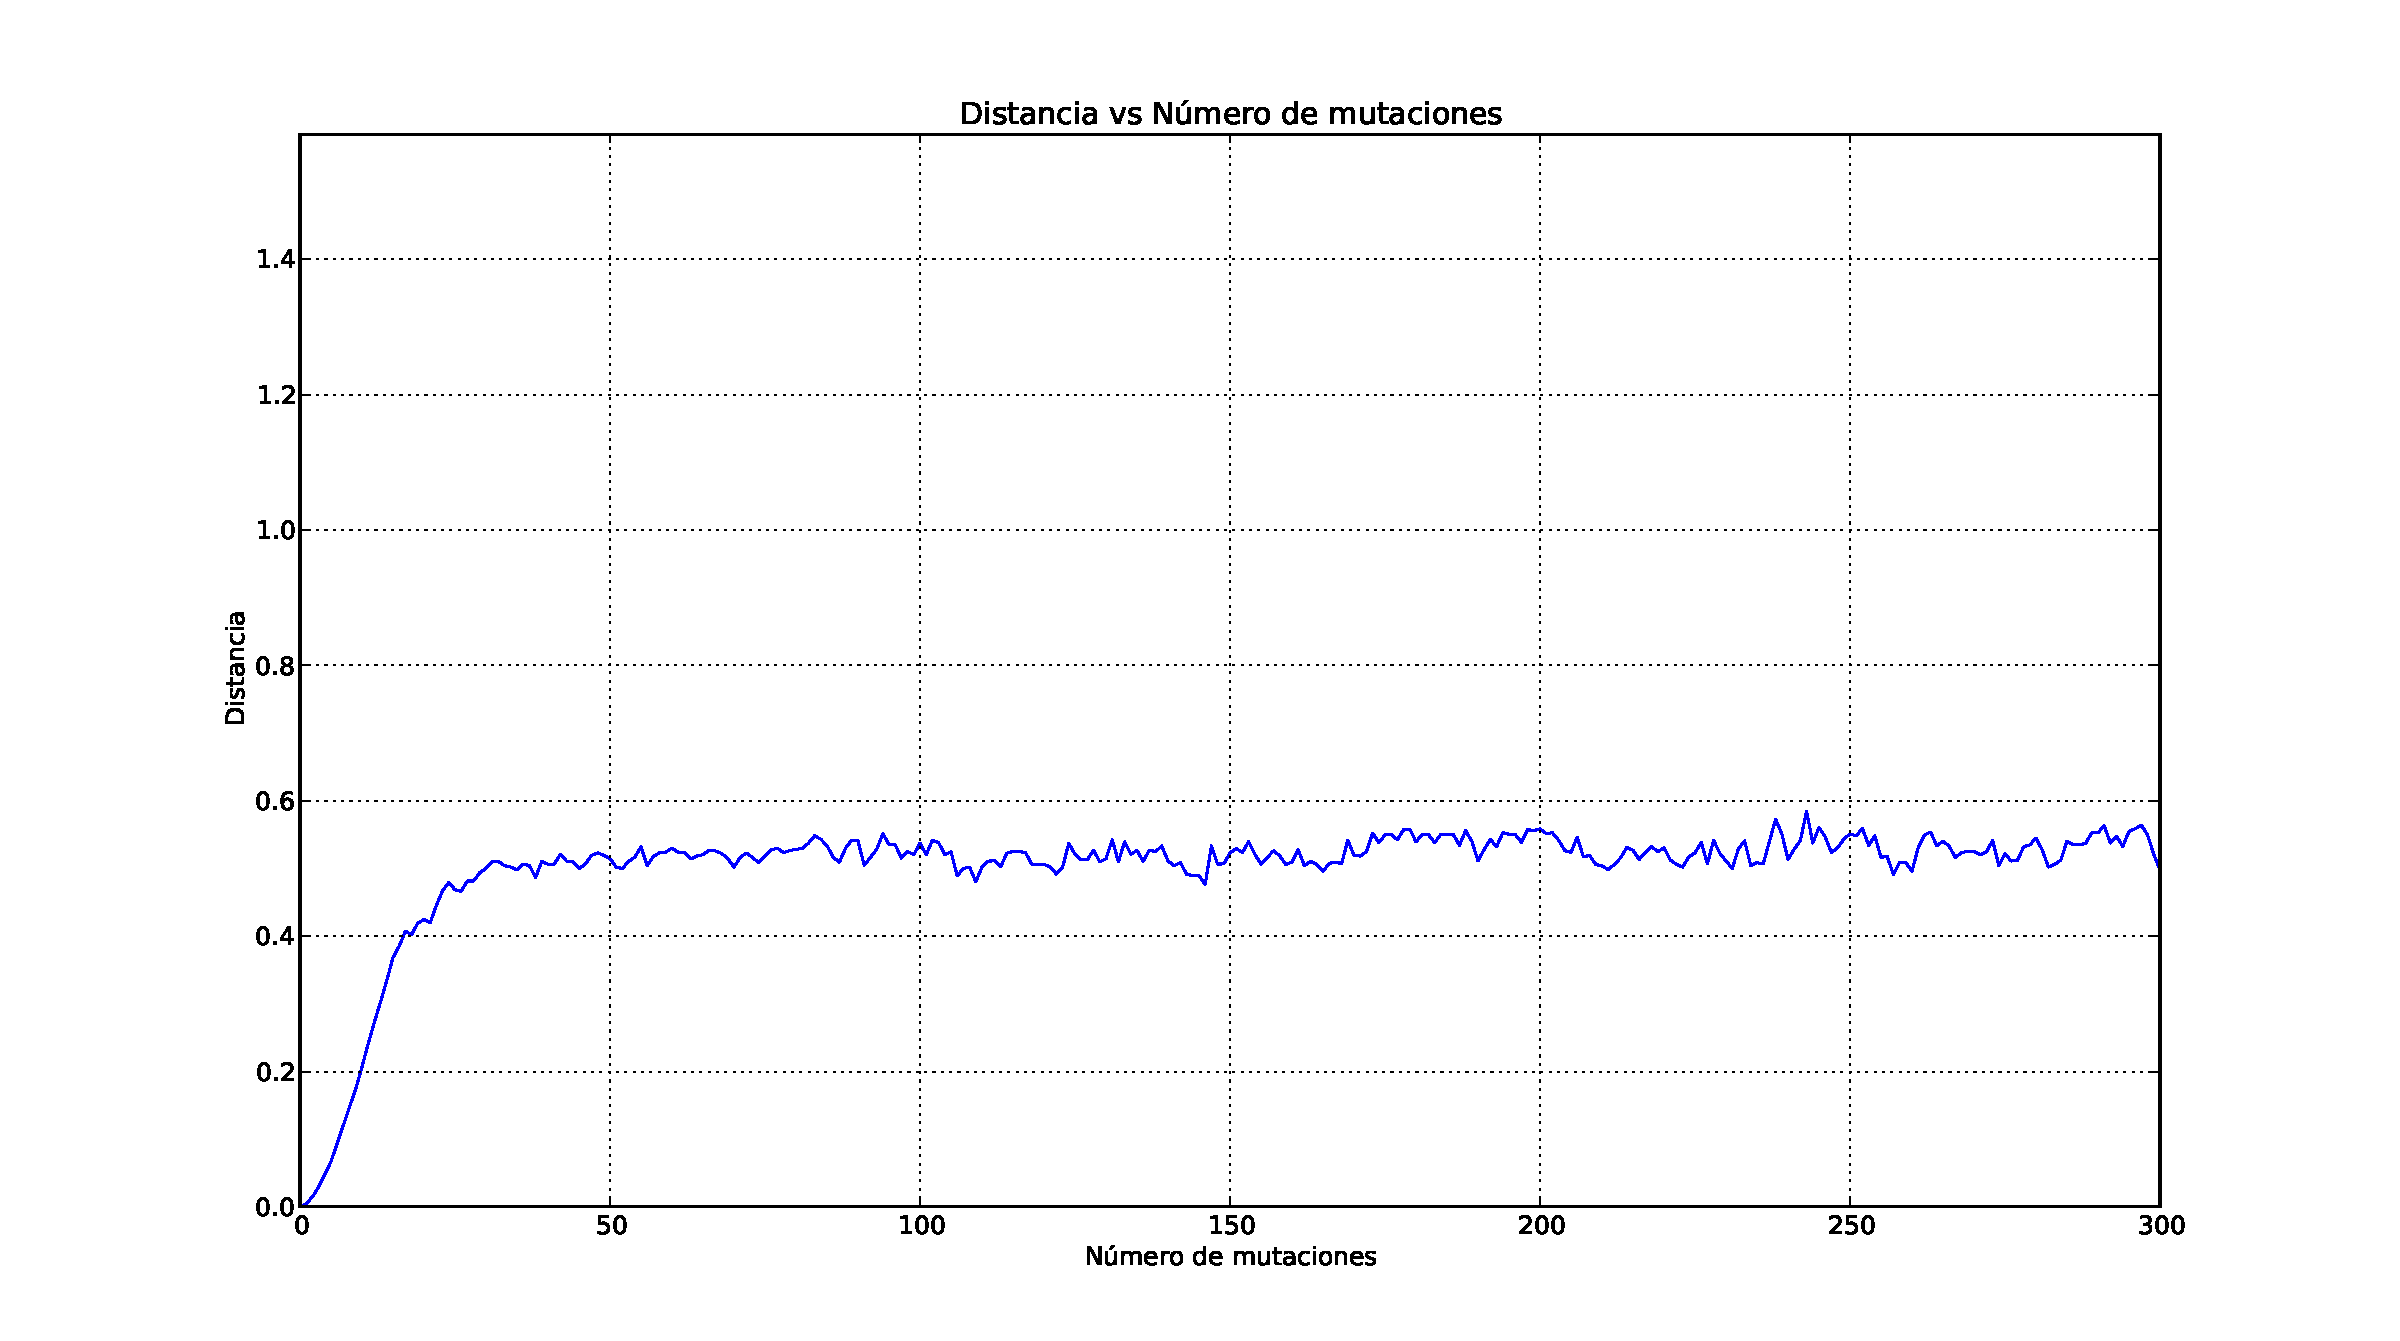
\includegraphics[width=\textwidth]{scripts/pregunta-2-1-new.pdf}
		\end{center}


	\item Genere una secuencia, clónela, y a cada copia aplíquele M mutaciones (de modo que tendrá
		dos secuencias crecientemente distintas). Grafique la relación entre M y D’, donde D’ es la
		distancia entre las dos secuencias que están mutando.

		\blue{Respuesta:}

		\begin{center}
			\includegraphics[width=\textwidth]{scripts/pregunta-2-2-new.pdf}
		\end{center}


	\item Genere 10.000 pares de secuencias (largo 200 c/u) y evalúe su distancia de Levenshtein; haga
		un histograma de la distribución de estos valores, y calcule media y $\sigma$

		\blue{Respuesta:}

		\begin{center}
			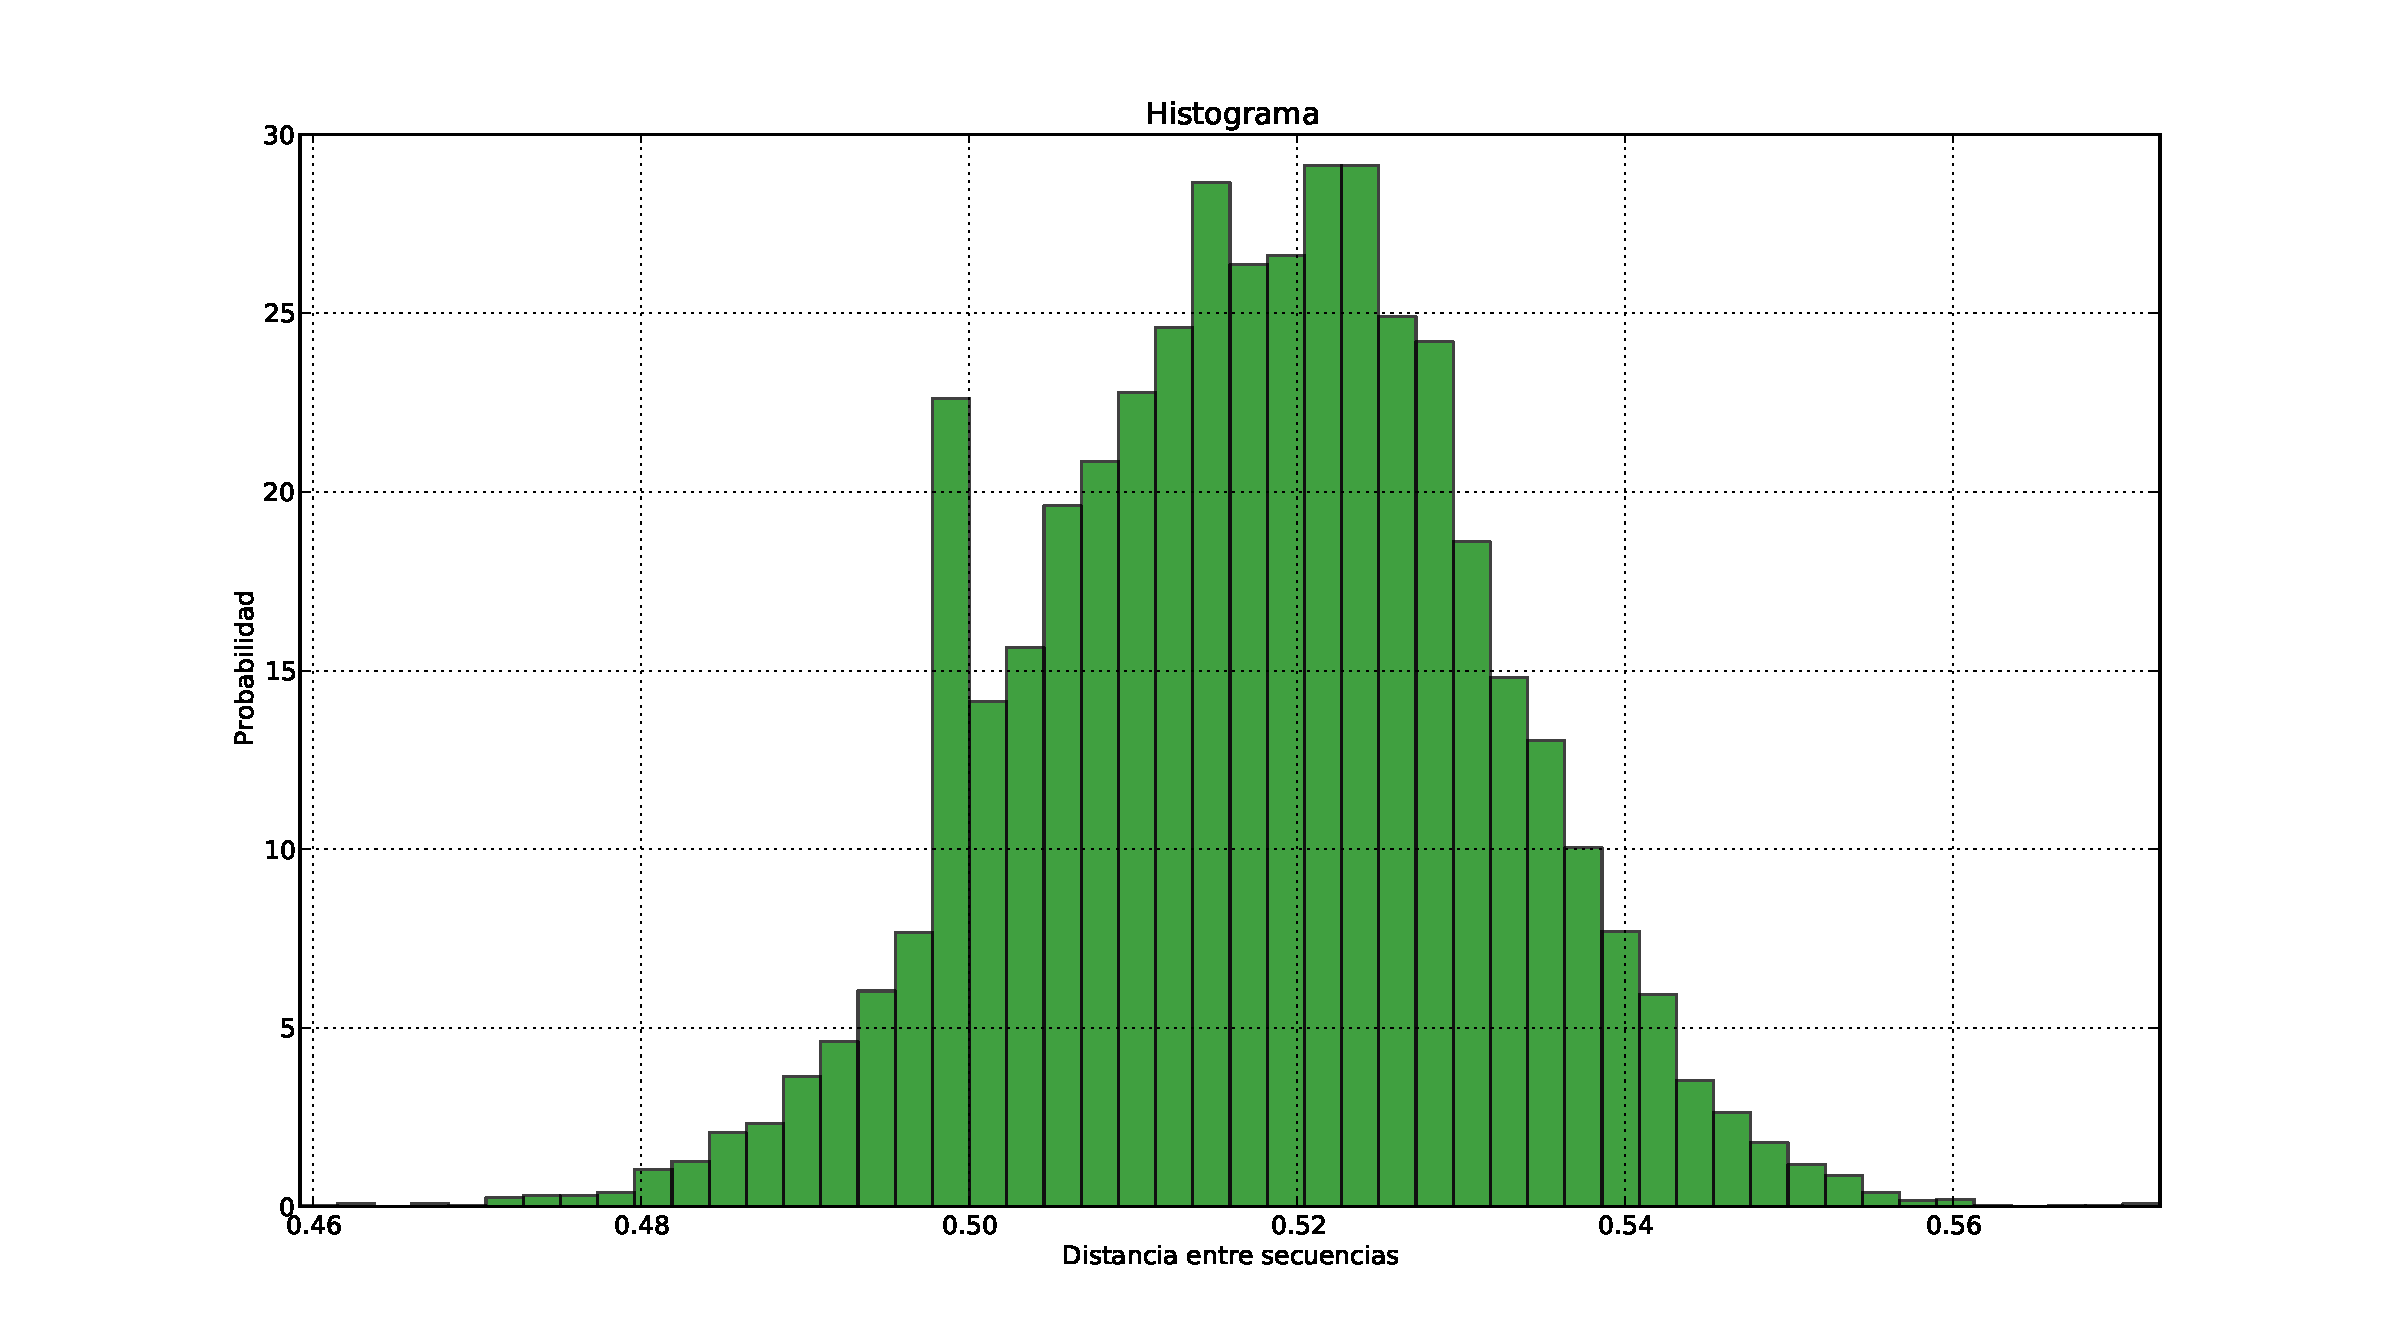
\includegraphics[width=\textwidth]{scripts/pregunta-2-3-new.pdf}
		\end{center}

		La información correspondiente del histograma y la aplicación es la siguiente:

		\begin{center}
		\begin{tabular}{|l|c|}
		\hline
		Largo 			 & 10000   \\\hline
		Media  			 & 0.517 \\\hline
		$\sigma$ 		 & 0.014   \\\hline
		Menor distancia  & 0.459   \\\hline
		Mayor distancia  & 0.573   \\\hline
		Tiempo ejecución & 4140.56 [sec] \\\hline
		\end{tabular}
		\end{center}

	\item Considerando (b) y (c), ¿por sobre qué valor de M diría usted que el parentesco entre las
		secuencias es indetectable?

		\blue{Respuesta:}

		Tomando en cuenta de que cada pregunta tiene sólo la idea central en común,
		es decir calcular la distancia de Levenshtein, pero después de todo,
		los ejercicios son distintos, pues el primero tiene que ver en ir comparando
		dos secuencias que van mutando en conjunto, y el segundo en 10000 pares de
		secuencias independientes que van mutando.

		La información que nos entregará cada ejercicio es la siguiente:
		\begin{itemize}
			\item \emph{(b):} Distancia entre dos secuencias a medida que se van mutando.
			\item \emph{(c):} Distribución de las distancias obtenidas entre 10000 pares de
				secuencias.
		\end{itemize}

		En el caso de la parte \emph{(b)} podemos ver que hasta las \red{30 mutaciones}
		hay una especie de crecimiento lineal, pero luego el comportamiento se torna
		mucho más impreciso, por lo que vamos obteniendo valores en la distancia
		sobre \blue{0.4}, pero a pesar de ser valores distintos, van siguiendo un mismo
		comportamiento, que es muy similar a la función de logaritmo, por lo que podríamos
		decir que la distancia normalizada posee un comportamiento casi logarítmico.

		Por otro lado, en \emph{(c)} nos podemos ver que la mayor cantidad de distancias
		se encuentra entre \blue{0.49} y \blue{0.54}, por lo que podemos deducir, que
		comparando estas distancias obtenidas con el gráfico de la parte \emph{(b)},
		que sobre unas \red{40 mutaciones}, la distancia comienza a ser mayor,
		por lo cual ya no podremos detectar fácilmente el parentesco entre las secuencias,
		a pesar de que todas las distancias obtenidas son similares.

		Finalmente nos damos cuenta de que las distancias en el caso \emph{(c)} siguen
		una \emph{distribución normal}, a pesar de existir un valor extraño cercano al \emph{0.5}.


\end{enumerate}

\newpage
\section{Problema 3}
\begin{enumerate}

	\item Siga programando en su lenguaje favorito. Esta vez, haga un programa que reciba una
		secuencia de DNA y encuentre en ella los 10 palíndromes más largos (un palíndrome, en
		sentido clásico, es una palabra que se lee igual en orden inverso; en el caso de DNA, además se
		complementan las bases, de modo que ACCTGATCAGGT es un palíndrome.).

		\blue{Respuesta:}
		
		Ver anexo 2~\ref{sec:anexo2}

	\item Vaya a~\footnote{\url{http://www.ncbi.nlm.nih.gov/genomes/genlist.cgi?taxid=2g\&type=0\&name=Complete\%20Bacteria}}
		y elija un cromosoma de bacteria (en general corresponderán a genomas completos de las bacterias),
		de no menos de 1.000.000 nt. Aplíquele su programa de la parte (a).

		\textbf{Ojo:} aparte de los resultados, especifique bien (con link y código de acceso) la secuencia que usó.

		\blue{Respuesta:}
		\begin{itemize}
			\item Información General
				\begin{itemize}
					\item Organism: \emph{Anaplasma centrale str. Israel}~\footnote{\url{http://www.ncbi.nlm.nih.gov/Taxonomy/Browser/wwwtax.cgi?id=574556}}
					\item Name: \emph{chromosome}
					\item Accession: \emph{NC\_013532}~\footnote{\url{http://www.ncbi.nlm.nih.gov/sites/entrez?db=genome&cmd=Retrieve&dopt=Overview&list_uids=25444}}
					\item Lenght: \emph{1206806 nt}
					\item Proteins:	\emph{923}~\footnote{\url{http://www.ncbi.nlm.nih.gov/sites/entrez?db=genome&cmd=Retrieve&dopt=Protein+Table&list_uids=25444}}
					\item RNAs: \emph{40}~\footnote{\url{http://www.ncbi.nlm.nih.gov/sites/entrez?db=genome&cmd=Retrieve&dopt=Structural+RNA+Table&list_uids=25444}}
					\item Genes: \emph{982}~\footnote{\url{http://www.ncbi.nlm.nih.gov/sites/gene?term=NC_013532[accn]}}
					\item Create date: \emph{Nov 26 2009}
					\item Update date: \emph{Mar 23 2010}
				\end{itemize}
			\item Secuencia
				\begin{itemize}
					\item Anaplasma centrale str. Israel, complete genome (NCBI)~\footnote{\url{http://www.ncbi.nlm.nih.gov/nuccore/CP001759}},
						notar que es necesario habilitar en el panel derecho ``Customize view'' y habilitar ``Show sequence'',
						la que aparecerá al final de la página.\\

					\texttt{
					ORIGIN\\ 
		        1 gtgggggggt ttatgccttt agaacagcag actactgata actccaatcc tgggttgaaa\\
		      	61 aaaaactcac atgccaaggg cgccagagag ccaaacgatg agcgttggac cacaaacgat\\
				...\\
				1206721 cagacctgta taaatccgcc ggggttgatg atgcactgct catcaatcgg ggggatttgt\\
  				1206781 tcttttttgt cgtatgtatt caaaac\\
					//
					}
				\end{itemize}

			\item Aplicación:\\

				Aplicando nuestra implementación, los resultados obtenidos son los siguientes:

				\begin{itemize}
					\item \texttt{gggaccaaggggtggttataaccaccccttggtccc}
					\item \texttt{acgggacactatagtgtcccgt}
					\item \texttt{gctataattgcaattatagc}
					\item \texttt{ggcatcatgcatgatgcc}
					\item \texttt{gggatgcagctgcatccc}
					\item \texttt{agacgttggccaacgtct}
					\item \texttt{tgtttgtatatacaaaca}
					\item \texttt{tcagtaagcttactga}
					\item \texttt{caagattgcaatcttg}
					\item \texttt{tctttgccggcaaaga}
				\end{itemize}
		
				El problema fue que el encontrar los palíndromos tomó \texttt{19414.7 [sec]},
				lo que es bastante tiempo, pero considerando que la primera aplicación que se
				programó estuvo corriendo todo un día, sin obtener resultados, es mucho más
				óptima a nivel de tiempo,

				por otro lado, el ordenar todos los palíndromos encontrados, desde el más
				largo al más corto, se demoró \texttt{24 [sec]}, lo cual es un muy buen
				resultado, considerando que el archivo que tenía todos los palíndromos
				pesaba \texttt{4.3 M}.
	
		\end{itemize}

	\item Sugiera una estrategia, basada en Smith-Waterman, para realizar esta tarea si nos interesaran
		palíndromes aproximados, donde se permitan reemplazos o inserciones.

			\blue{Respuesta:}

			\red{TO DO:} Completar

			Se propone el siguiente procedimiento para llevar a cabo la búsqueda
			de palíndromos aproximada.

			\begin{enumerate}
				\item 
			\end{enumerate}
			


\end{enumerate}

\newpage
\section{Problema 4}
Retome las 6 proteínas encontradas en la tarea 1 (los primeros 6 matches que les dio BLAST)

\begin{enumerate}
	\item Alinee sus secuencias usando Clustal (www.clustal.org). Muestre el alineamiento. ¿Quedan
		alineados entre sí los segmentos que se alineaban con su nombre?
	
		\blue{Respuesta:}

		Se seleccionó 3 proteínas por cada integrante, como se señaló en la clase.

		\begin{tabular}{|l|l|}
			\hline
			GARIELAMRA & CRISTIANMAREIRA \\
			\hline
			ZP\_01751021.1 & EFO18319.1 \\ 
			YP\_001613385.1 & AAK08622.1 \\
			ZP\_05971288.1 & ZP\_05842161.1 \\
			\hline
		\end{tabular}

	El alineamiento puede verse en la sección anexos (4.1).	No quedan alineados los nombre.
			

	\item Corte, de cada secuencia, el segmento que se alinea con su nombre. Con las 7 secuencias,
		haga un nuevo alineamiento en Clustal.

		\blue{Respuesta:}

		Debido a que somos dos integrantes, tomaremos las 3 primeras secuencias encontraras por cada uno y el segmento GARIELAMRA.

	El alineamiento puede verse en la sección anexos (4.2).

	\item Usando ese alineamiento, construya y dibuje (“a mano”, es decir, sin usar software de HMM)
		un HMM.

		\blue{Respuesta:}

		\red{TO DO:} Completa.

	\item Determine la secuencia de estados internos más probable en ese HMM para emitir su
		nombre.

		\blue{Respuesta:}

		\red{TO DO:} Completa.

\end{enumerate}

\newpage
\section{Anexos}
% Agregar:
% antecedentes recolectados
% otros (imágenes, textos, tablas, etc.)




\subsection{Actividades y tiempos empleados por cada integrante}

\begin{tabular}{|l|p{7cm}|c|}
\hline
Integrante & Actividades & Tiempo Empleado \\\hline
Cristián Maureira & Observación de los medios de comunicación y reuniones internacionales. & 7 horas \\
& Creación del Repositorio de trabajo. & 30 minutos \\
& Creación del esqueleto del informe.& 30 minutos \\
& Desarrollo de la introducción. & 2.5 horas \\
& Redacción de los análisis y resultados de antecedentes. & 3 horas \\
& Revisión de los análisis y resultados de antecedentes. & 1 hora \\
\hline
Gabriel Zamora & Revisión de  las formas de trabajo de cada grupo. & 8 horas \\
& Estudio del público objetivo y del dominio del trabajo. & 3 horas \\
& Redacción de los análisis y resultados de antecedentes. & 4 horas \\
\hline
Rodrigo Fernández & Comparación de los resultados con los antecedentes
recopilados. & 5 horas \\
& Investigación de la información existente. & 5 horas \\
& Redacción de los análisis y resultados de antecedentes. & 3 horas \\
& Revisión del análisis y resultados de antecedentes. & 30 minutos \\
& Revisión ortográfica del informe. & 10 minutos \\
\hline
\end{tabular}
\newpage
\subsection{Participantes de las reuniones}
\subsubsection{OSF Coordination Meeting}

\begin{tabular}{|l|l|l|l|}
	\hline
	{\bf Nombre} & {\bf Cargo} & {\bf Organización} & {\bf País} \\\hline
	Heiko Sommers & ACS Technical Leader & ESO & Alemania \\\hline
	Gianluca Chiozzi & ESO Astronomical Instrumentation Leader & ESO & Italia \\\hline
	Alessandro Caproni & Software Engineer& ESO & Italia \\\hline
	Matias Mora & Software Engineer & ALMA & Chile \\\hline
	Nicolas Troncoso & Software Engineer & ALMA & Chile \\\hline
	Jorge Avarias & Software Engineer & NRAO & EEUU \\\hline
	Rodrigo Tobar & Software Engineer & ESO & Alemania \\\hline
	Jaime Pavlich & Profesor & UCN & Chile \\\hline
	Tomas Staig & Computer Science Student & UTFSM/ESO & Chile \\\hline
	Arturo Hoffstadt & Computer Science Engineer & UTFSM/NRAO & Chile \\\hline
	Gabriel Zamora & Computer SCience Student & UTFSM & Chile \\\hline
	Cristián Maureira & Computer SCience Student & UTFSM & Chile \\\hline	
\end{tabular}

\subsubsection{ACS Weekly Meeting}

\begin{tabular}{|l|l|l|l|}
	\hline
	{\bf Nombre} & {\bf Cargo} & {\bf Organización} & {\bf País} \\\hline
	Joseph Schwarz & ACS Project Leader & ESO & Alemania \\\hline
	Heiko Sommers & ACS Technical Leader & ESO & Alemania \\\hline
	Gianluca Chiozzi & ESO Astronomical Instrumentation Leader & ESO & Italia \\\hline
	Alessandro Caproni & Software Engineer& ESO & Italia \\\hline
	Jorge Avarias & Software Engineer & NRAO & EEUU \\\hline
	Rodrigo Tobar & Software Engineer & ESO & Alemania \\\hline
	Arne Grimstrup & Software Engineer & NRAO & Canada \\\hline
	Bogdam Jeram & Software Engineer & ESO & Eslovenia \\\hline
	Helmut Tischer & Software Engineer & ESO & Alemania \\\hline
	Matej Sekoranja & Software Engineer  & ESO & Eslovenia \\\hline
	Roberto Cirami & Software Engineer & INAF - OAT & Italia\\\hline
	Tomas Staig & Computer Science Student & UTFSM/ESO & Chile \\\hline
	Gabriel Zamora & Computer Science Student & UTFSM & Chile \\\hline
	Cristián Maureira & Computer Science Student & UTFSM & Chile \\\hline	
\end{tabular}

% CORRECCION 6
\subsubsection{Fotografías}
A continuación se muestran algunas fotografías tomadas mientras se realizaban las reuniones semanales.\\

\begin{center} 
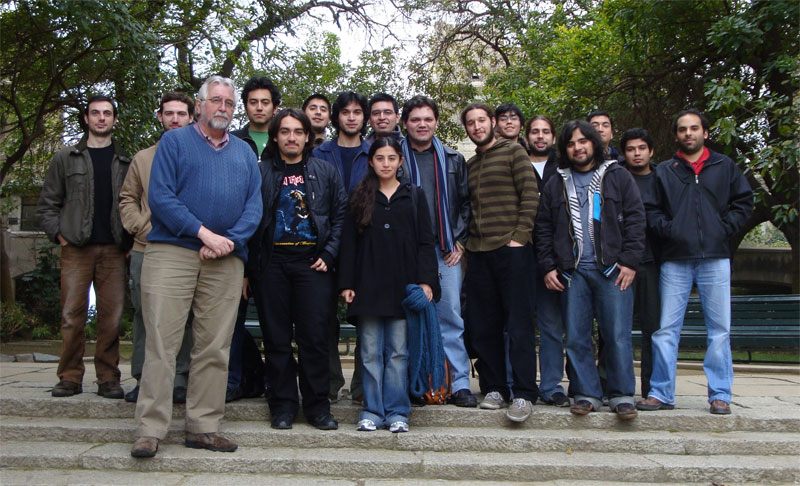
\includegraphics[width=0.8\textwidth]{images/alma-utfsm-1}\\\vspace{1cm}
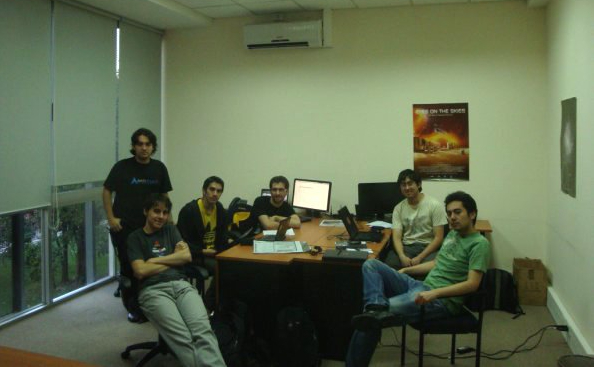
\includegraphics[width=0.8\textwidth]{images/alma-utfsm-2}\\
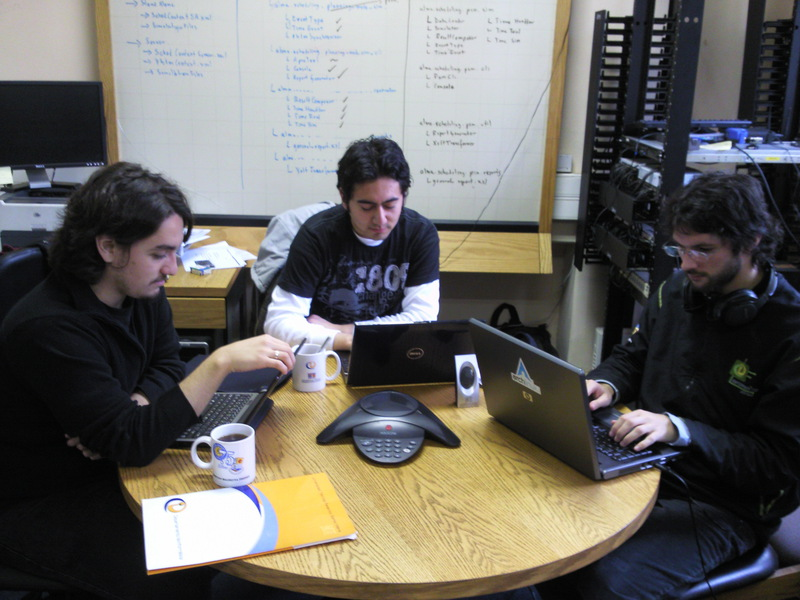
\includegraphics[width=0.8\textwidth]{images/lab_conference}\\\vspace{1cm}
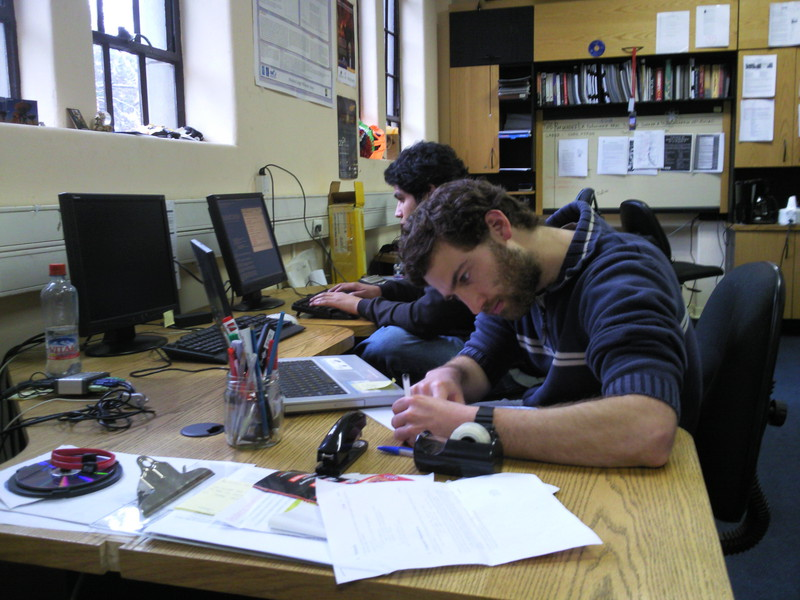
\includegraphics[width=0.8\textwidth]{images/lab_working}\\
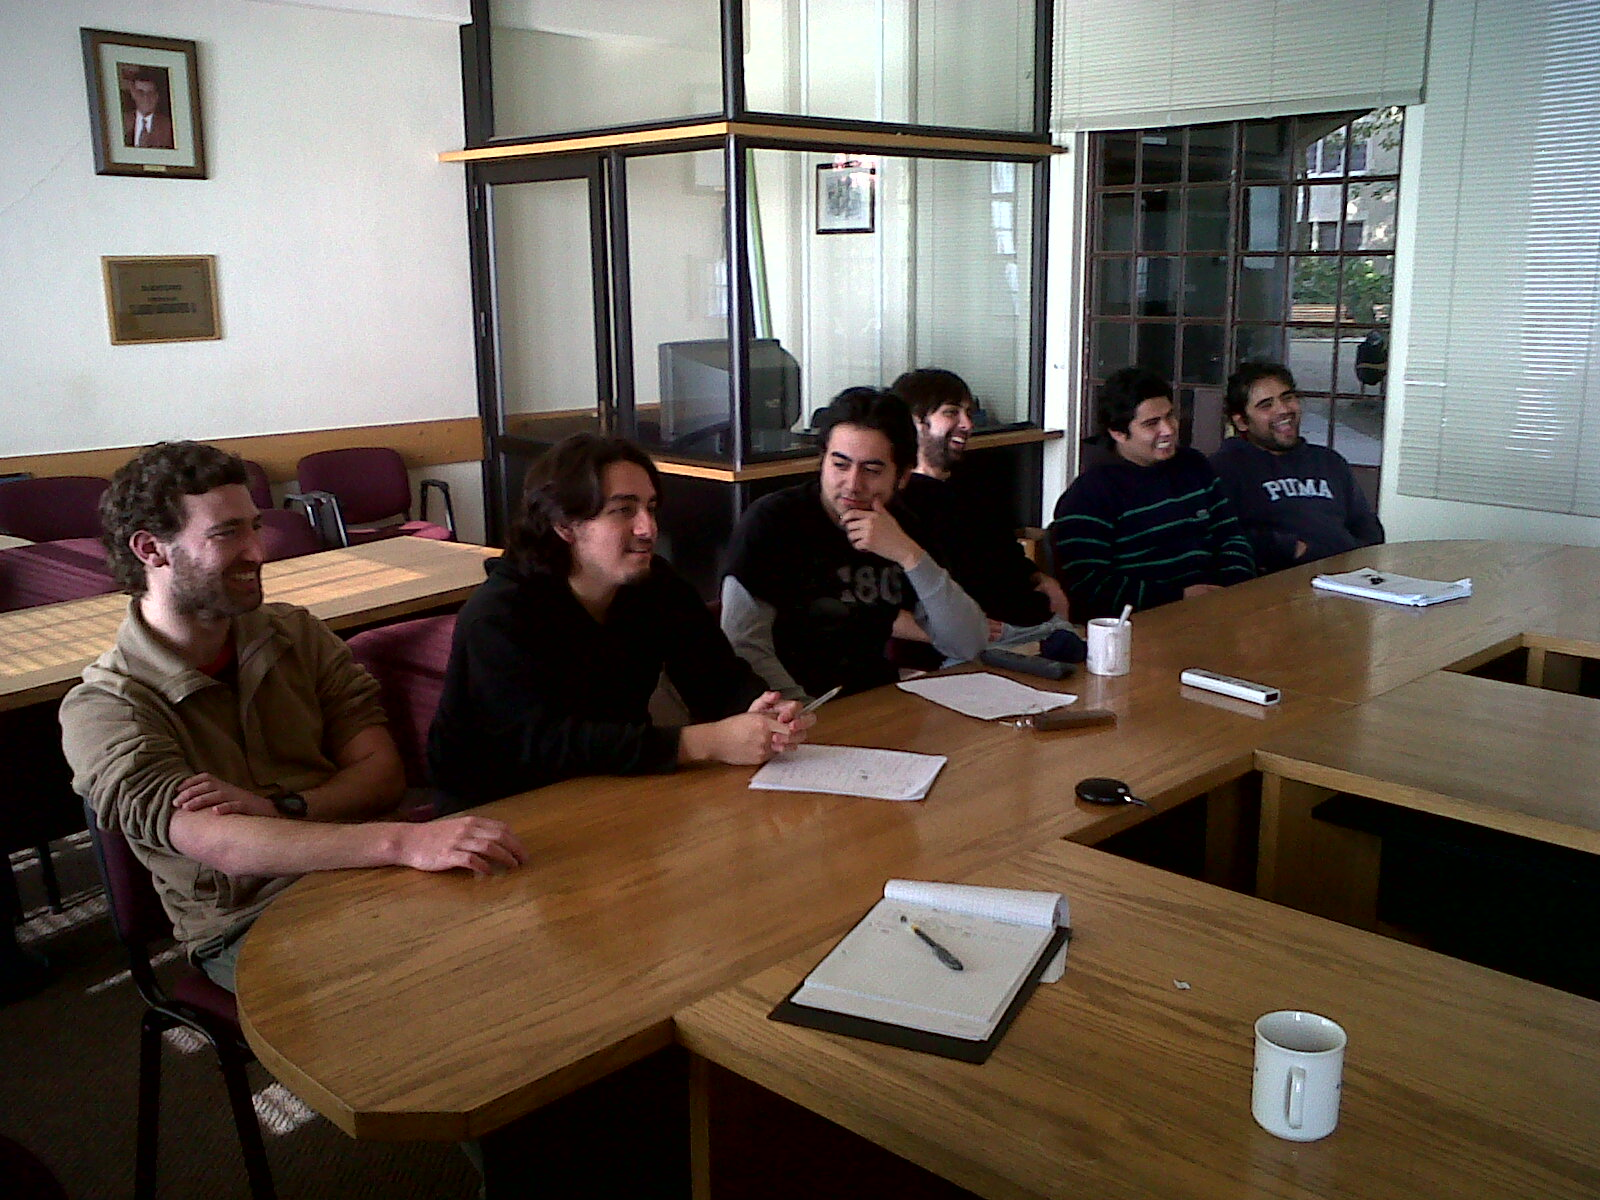
\includegraphics[width=0.8\textwidth]{images/leads1}\\\vspace{1cm}
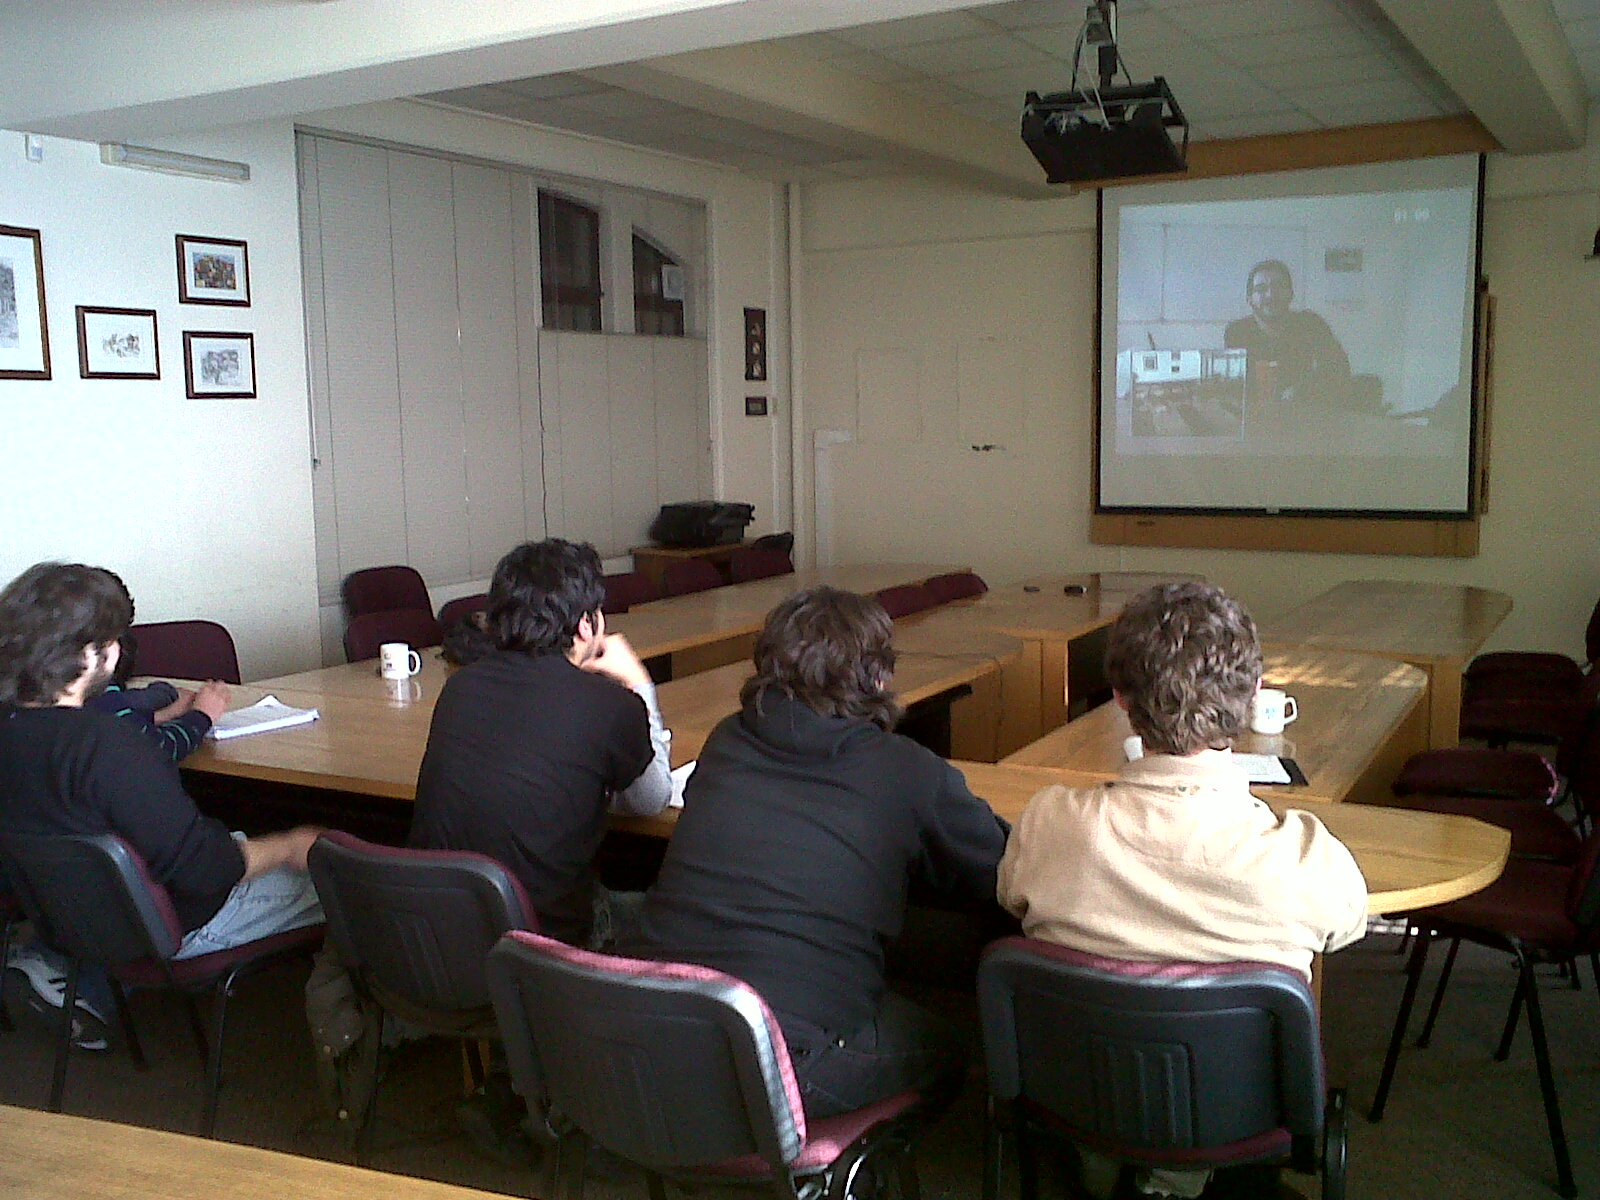
\includegraphics[width=0.8\textwidth]{images/leads2}
\end{center}
% CORRECCION &

\newpage
\subsection{Minutas de reuniones}
\subsubsubsection{ACS Weekly Meeting}
\begin{verbatim}
ACS Weekly Phone Meeting 
Date: Monday, 2010-04-12 

Attendees: 
ESO: Bogdan, Gianluca, Heiko, JosephSchwarz, 
NRAO: ArneGrimstrup, JorgeAvarias 
JSI: 
AOT: 
ALMA Chile: Ale 
UTFSM: GabrielZamora CristianMaureira 

Control contact number: +1-203-607-6471 (Passcode 203403#) 

General issues 

Alma has a promising candidate for a new board to replace the VMEs with 64 
bit architecture, to support more memory. Details from Thomas J. 
All module owners please fix their tests on 8.2 branch and HEAD. 

Ale Caproni 

Last week: 

CONTROL: Some issues with TotalPower testing, also due to STEs gotten messed up 
by other testers. 
The TP component has been changed to use the C++ API of the Bulk data libs, 
without reusing the IDL wrapper of the bulk data component. This works fine 
now, but still would like to discuss changes to the BD IDL for the long term. 
Will be at ESO early May. Things to be discussed should be added to Ale's 
Main.May2010 page.

Arne Grimstrup 

Last week: 

Continued investigation of COMP-3072 (with J. Avarias) 
problem still occurs with RHEL 5.4 version of CASA 
select is monitoring a bad file descriptor which triggers an exception 
in the TAO code. Telecon with UTFSM regarding future projects 
(with G. Chiozzi, H. Sommer, et. al.) Support 
Investigation of 64-bit test faults in NRI (H. Sommer)(with J. Avarias) 
Template method was invoking unsigned long version of getValue method 
that didn't exist Documentation for generated Python bindings (J. Kern) 
Questions regarding Python Binding Generator (J. Kern) 
Problem building ACS in INTROOT (J. Avarias) 

This week: 
Continue work on COMP-3072 
Continue work on COMP-830 

Bogdan Jeram 

Last week: 
Monday public holiday 
4 days of vacation 

Heiko Sommer 

Last week: 

Worked out HibernateDAL's usage of Archive's new archiveConfig.properties 
mechanism, together with Holger. 
Finalized 8.1 CVS logs and release notes. Pre-release of 9.0 VM. 
Discussions, e.g. TP with Ale and others 
Support, e.g. XSD validation, CDB performance fix, manager error messages, 
1 day leave 
Telecon with UTFSM about current projects 
quarterly report for ESO 

Helmut Tischer 

Last week: 
Vacation 

This week: 
COMP-2214 continuing 

Joe Schwarz 

Last week: 

Discussed problem of simultaneous use of SB by > 1 STE; change in 
lifecycle-handling needed 
Reviewed FP6 quarterly report from U. of Cambridge 
Worked on Total Power crash of Java container; suggested JNI 
debugging options for JVM runtime to Jeff and Ville, also removing
 native method invocation from class constructor (this didn't 
make any difference, however); got help from Roberto, who looked 
at logs and said he saw no bulk data issues 
Discussed CDR8 preparations w/Heiko 
Tried (and failed) to convince Brian to take Observation Control 
(not yet delivered) out of R7.1 
One day's leave 

This week: 
CDR8 preparation, ACS 9.0 planning 
Continue investigation of Total Power problem 
Return to classpath generation 

Jorge Avarias 

Last week: 

COMP-3749: ACS to introduce a new log level between DEBUG and TRACE 
Finished to make the last changes to the tests (Changed ACS_LOG_STDOUT 
from 2 to 1 new trace) 
All the tests affected by this are passing. 
Continued investigation of COMP-3072 (with A, Grimstrup) 
Fixed NRI ACS 64 bits building problems: 
The method unsigned long cdb::DAONode::getValue(char const*) 
was missing. probably some code is using unsigned long instead 
CORBA::ULong (in 32 bits they have the same length, in 64 they have not) 
Support: 
CONTROL/ACC/cppContainer crash (T. Powers) 
CONTROL/ACC/javaContainer crash, JVM is crashing with Seg. Fault 
(J. Kern, V. Suoranta) 
Problems building ACS in INTROOT (ACS is already built in ACSROOT) 
(S. Rankin) 


Matej Sekoranja 

Last week: 
HibernateDAL now skips loading all .dtd files, XMLSchema.xsd and xml.xsd so 
that Oracle's XMLTYPE checks don't get confused. 

This week: 
At CERN, but available for emergency ACS work. 

This week: 
TMCDB integration at the OSF 

UTFSM 

Last week: 

DDS Logging Service 
All the main goals are completed 
There are one pending task, write a "state of art" in this topic, for the paper 
accepted in the SPIE Meeting with people at ESO to define project objectives. 
Planning
Python support for BACI Properties 
ACS Code Generation 
ACS Windows Porting (Rodrigo and Heiko to integrate Java porting, Camillo and 
Gianluca to continue with C++ porting)
\end{verbatim}
\newpage
\subsubsubsection{OSF Coordination Meeting}

\begin{verbatim}
Date: Tue, 2010-05-18, 11:00 Chile, 9:00 Socorro, 17:00 Germany 
Attendees: 

ALMA-Chile: MatiasMora 
NRAO-Socorro: JorgeAvarias 
ESO-Garching: HeikoSommers 
UTFSM: GabrielZamora, TomasStaig, ArturoHoffstadt, CristianMaureira 
UCN: JaimePavlich 

Contact Info 
When: 11:00 Chile / 9:00 NM / 17:00 Germany 
Chile (toll free): 800532833 
International: +1 3032480281 
Access Code: 4676238 
Web Conferencing URL: http://net.globalcrossing.com/conferencing/ 

Agenda 
ALMA-CONICYT #31090034 (UTFSM) 
Projects 
ACS Windows Porting: The first version of the gcc-wrapper (gcc -> cl) is 
ready, we need to test with real examples to improve it. 
Code Generation: Luigi sent us a project proposal. Because Luigi was on
 vacations the last week, the meeting for this project is pending 
Alarms Configuration GUI: 
The project is ready, but there are some details with the redaction. 
Rules view that Tomas will fix in the week. 
Cristian Maureira and Tomas Staig will work on the documentation the 
next week. 
Official acceptance by ACS. 
Sampling System GUI: 
Juan Reyes and Cristian Maureira closed two of the three pending bugs, 
there are only one pending, that will be ready during the week. 
Official acceptance by ACS. 
ALMA-CONICYT #31080031 (AIA) 
Teams working on papers and on a new task about implementing TSP with 
their paper techniques 
HPC must to define the input framework and do some testing with TSP 
SebastianDuran and WalterFarina will be helping MatiasMora on what 
he needs for his thesis 
Second class this week Valpo. and next week Stgo. about advanced 
AI techniques 
Looking for possibilities of collaborations with MAIA-INRIA 
Summer Jobs 2010 
Pending reports! 
UCN Current Status 
Mini-ACS-Workshop from April 27th to May 10th. Funded by 
ALMA #31090026. 
Repository for UCN projects: http://goos-acs.googlecode.com 
gCCD status 
Implementing support for SBIG cameras 
Moving configuration to CDB 
gDome status 
gDome group are new students. After several intensive sessions 
they created the first version of the Dome component. 
Documentation: installation and system manuals. 
Misc 
ACS Scientific Linux distribution mirror repo here at UTFSM (ArturoHoffstadt).
\end{verbatim}


\end{document}
